\documentclass{bioinfo}

\usepackage{url}
\usepackage{multirow}
\usepackage{authblk}
\usepackage{rotating}
\usepackage{xr}
\usepackage{amsfonts}
\usepackage{amsmath}
\usepackage{algorithm}
\usepackage[noend]{algpseudocode}

\newcommand{\todo}[1]{}

% added from http://tex.stackexchange.com/questions/78776/forced-indentation-in-algorithmicx to help with wrapping lines in algorithmic enviro
\makeatletter
\newlength{\continueindent}
\setlength{\continueindent}{6em}

\renewenvironment{algorithmic}[1][0]%
   {%
   \edef\ALG@numberfreq{#1}%
   \def\@currentlabel{\theALG@line}%
   %
   \setcounter{ALG@line}{0}%
   \setcounter{ALG@rem}{0}%
   %
   \let\\\algbreak%
   %
   \expandafter\edef\csname ALG@currentblock@\theALG@nested\endcsname{0}%
   \expandafter\let\csname ALG@currentlifetime@\theALG@nested\endcsname\relax%
   %
   \begin{list}%
      {\ALG@step}%
      {%
      \rightmargin\z@%
      \itemsep\z@ \itemindent\z@ \listparindent2em%
      \partopsep\z@ \parskip\z@ \parsep\z@%
      \labelsep 0.5em \topsep 0.2em%\skip 1.2em 
      \ifthenelse{\equal{#1}{0}}%
         {\labelwidth 0.5em}%
         {\labelwidth 1.2em}%
       \leftmargin\labelwidth \addtolength{\leftmargin}{\labelsep}
      \ALG@tlm\z@%
      }%
      \parshape 2 \leftmargin \linewidth \continueindent \dimexpr\linewidth-\continueindent\relax
   \setcounter{ALG@nested}{0}%
   \ALG@beginalgorithmic%
   }%
   {% end{algorithmic}
   % check if all blocks are closed
   \ALG@closeloops%
   \expandafter\ifnum\csname ALG@currentblock@\theALG@nested\endcsname=0\relax%
   \else%
      \PackageError{algorithmicx}{Some blocks are not closed!!!}{}%
   \fi%
   \ALG@endalgorithmic%
   \end{list}%
   }%
\makeatother

%\externaldocument[S]{supplementary}

\copyrightyear{2014}
\pubyear{2014}

\begin{document}
\firstpage{1}

\title[Cloudbreak]{Cloudbreak: Accurate and Scalable Genomic Structural Variation Detection in the Cloud with MapReduce}
\author[Whelan \textit{et~al}]{Christopher W. Whelan\,$^{1}$, Jeffrey Tyner\,$^{2}$, Alberto L'Abbate\,$^{3}$, Clelia Tiziana Storlazzi,$^{3}$, Lucia Carbone\,$^{4}$, and Kemal S\"onmez\,$^{1,5,*}$\footnote{to whom correspondence should be addressed}}
\address{$^{1}$Institute on Development and Disability and Center for Spoken Language Understanding, Oregon Health \& Science University (OHSU), Portland, OR, USA \\
$^{2}$ Program in Molecular and Cellular Biosciences, OHSU\todo{Oregon Health \& Science University}, Portland, OR, USA \\
$^{3}$ Department of Biology, University of Bari ``Aldo Moro'', Via G. Amendola 165/A, 70126, Bari, Italy \\
$^{4}$ Behavioral Neuroscience Department, OHSU\todo{Oregon Health \& Science University}, Portland, OR, USA \\
$^{5}$ Department of Medical Informatics \& Clinical Epidemiology, OHSU\todo{Oregon Health \& Science University}, Portland, OR, USA 
}

\history{Received on XXXXX; revised on XXXXX; accepted on XXXXX}

\editor{Associate Editor: XXXXXXX}

\maketitle

\begin{abstract}

\section{Motivation:}
The detection of genomic structural variations (SV) remains a difficult challenge in analyzing sequencing data, and the growing size and number of sequenced genomes have rendered SV detection a bona fide big data problem. MapReduce is a proven, scalable solution for distributed computing on huge data sets.

\section{Results:}
We describe an algorithmic framework for SV detection algorithms in MapReduce based on computing local genomic features, and use it to develop a deletion and insertion detection algorithm, Cloudbreak. On simulated and real data sets, Cloudbreak achieves accuracy improvements over popular SV detection algorithms, and genotypes variants from diploid samples. It provides dramatically shorter runtimes and the ability to scale to big data volumes on large compute clusters. Cloudbreak includes tools to set up and configure MapReduce (Hadoop) clusters on cloud services, enabling on-demand cluster computing.

\section{Availability:}
Source code, binary releases, and user manual are available at \url{http://github.com/cwhelan/cloudbreak}

\section{Supplementary information:} Supplementary material is available at \emph{Bioinformatics} online.

\section{Contact:} \href{sonmezk@ohsu.edu}{sonmezk@ohsu.edu}
\end{abstract}

\section{Introduction}

Genomic structural variations (SVs) such as deletions, insertions, and inversions of DNA are widely prevalent in human populations and account for the majority of the bases that differ among normal human genomes~\citep{Mills:2011p1611, Conrad:2010ja}. However, detection of SVs with current high-throughput sequencing technology remains a difficult problem, with limited concordance between available algorithms and high false discovery rates~\citep{Mills:2011p1611}. Part of the problem stems from the fact that the signals indicating the presence of SVs are spread throughout large data sets, making the problem computationally intensive. As the volume of massively parallel sequencing data approaches ``big data'' scales, SV detection is becoming a time consuming component of genomics pipelines, and presents a significant challenge for research groups and clinical operations that may not be able to scale their computational infrastructure. Here we present a distributed software solution that is scalable and readily available on the cloud.

In other fields that have taken on the challenge of handling very large data sets, such as internet search, scalability has been addressed by frameworks that distribute processing to many compute nodes, each working on local copies of portions of the data. In particular, Google's MapReduce~\citep{Dean:2008p277} was designed to manage the storage and efficient processing of big data across clusters of commodity servers. Hadoop is an open source project of the Apache Foundation that provides an implementation of MapReduce. MapReduce and Hadoop allow efficient processing of large data sets by executing tasks on nodes that are as close as possible the data they require, minimizing network traffic and I/O contention. The Hadoop framework has been successfully applied to sequencing-related tasks including short read mapping~\citep{Schatz:2009p278} and SNP calling~\citep{Langmead:2009p1225}.

Hadoop/MapReduce requires a specific programming model, however, which can make it difficult to design general-purpose algorithms for arbitrary sequencing problems like SV detection. MapReduce divides computation across a cluster into three phases. In the first phase, \emph{mappers} developed by the application programmer examine small blocks of data and emit a set of $\langle key, value \rangle$ pairs for each block examined. The framework then sorts the output of the mappers by key, and aggregates all values that are associated with each key. Finally, the framework executes \emph{reducers}, also created by the application developer, which process all of the values for a particular key and produce one or more outputs that summarize or aggregate those values.

SV detection algorithms use three main signals present in high-throughput sequencing data sets~\citep{Alkan:2011p547}. Read-pair (RP) based methods use the distance between and orientation of the mappings of paired reads to identify the signatures of SVs~\citep{Campbell:2008p539,Chen:2009p3,Sindi:2009gu,Korbel:2009dy}. Traditionally, this involves separating mappings into those that are \emph{concordant} or \emph{discordant}, where discordant mappings deviate from the expected insert size or orientation, and then clustering the discordant mappings to find SVs supported by multiple discordantly mapped read pairs. Read-depth (RD) approaches consider the changing depth of coverage of concordantly mapped reads along the genome~\citep{Alkan:2009cr,Yoon:2009kb,Chiang:2009di}. Finally, split-read (SR) methods look for breakpoints by mapping portions of individual reads to different genomic locations~\citep{Wang:2011p1607,Ye:2009p2}.

Many RP methods consider only unambiguously discordantly mapped read pairs. Some approaches also include ambiguous mappings of discordant read pairs to improve sensitivity in repetitive regions of the genome~\citep{Hormozdiari:2009p284,Quinlan:2010gf}. Several recent RP approaches have also considered concordant read pairs, either to integrate RD signals for improved accuracy~\citep{Sindi:2012kk,Michaelson:2012fj,Chiara:2012ey}, or to eliminate the thresholds that separate concordant from discordant mappings and thus detect smaller events~\citep{Marschall:2012ek}. Increasing the number of mappings considered, however, increases the computational burden of SV detection. 

Our goal is to leverage the strengths of MapReduce to provide fast, accurate and readily scalable SV-detection pipelines. The main challenge in this endeavor is the need to separate logic into mappers and reducers, which makes it difficult to implement traditional RP-based SV detection approaches in MapReduce, particularly given the global clustering of paired end mappings at the heart of many RP approaches. MapReduce algorithms, by contrast, excel at conducting many independent calculations in parallel. In sequencing, for example, MapReduce based SNV-callers Crossbow~\citep{Langmead:2009p1225} and GATK~\citep{McKenna:2010p1051} perform independent calculations on partitions of the genome. SV approaches that are similarly based on local computations have been described: the RP-based SV callers MoDIL~\citep{Lee:2009da} and forestSV~\citep{Michaelson:2012fj} compute features along the genome and then produce SV predictions from those features in a post-processing step. We will show that this strategy can be translated into the MapReduce architecture.

In this paper, we describe a framework for solving SV detection problems in Hadoop based on the computation of local genomic features from paired end mappings. We have used this framework to develop a software package, Cloudbreak, that discovers genomic deletions up to 25,000bp long, and short insertions. Cloudbreak computes local features based on modeling the distribution of insert sizes at each genomic location as a Gaussian Mixture Model (GMM), an idea first implemented in MoDIL~\citep{Lee:2009da}. The use of Hadoop enables scalable implementations of this class of algorithm. We characterize our algorithm's performance on a simulated data set, as well as a high coverage real data set from a normal individual and a low coverage cancer data set, and compare its performance to those of several popular methods. 

Finally, and quite importantly from a practical point of view, our implementation of Cloudbreak provides the functionality to easily set up and configure Hadoop clusters on cloud service providers, making dynamically scalable distributed SV detection accessible to all whose computational needs demand it.

% \begin{equation}
% \sum x+ y =Z\label{eq:01}
% \end{equation}

\begin{methods}
\section{Methods}

\subsection{A Framework for SV Detection in MapReduce}

\begin{figure}
\centering
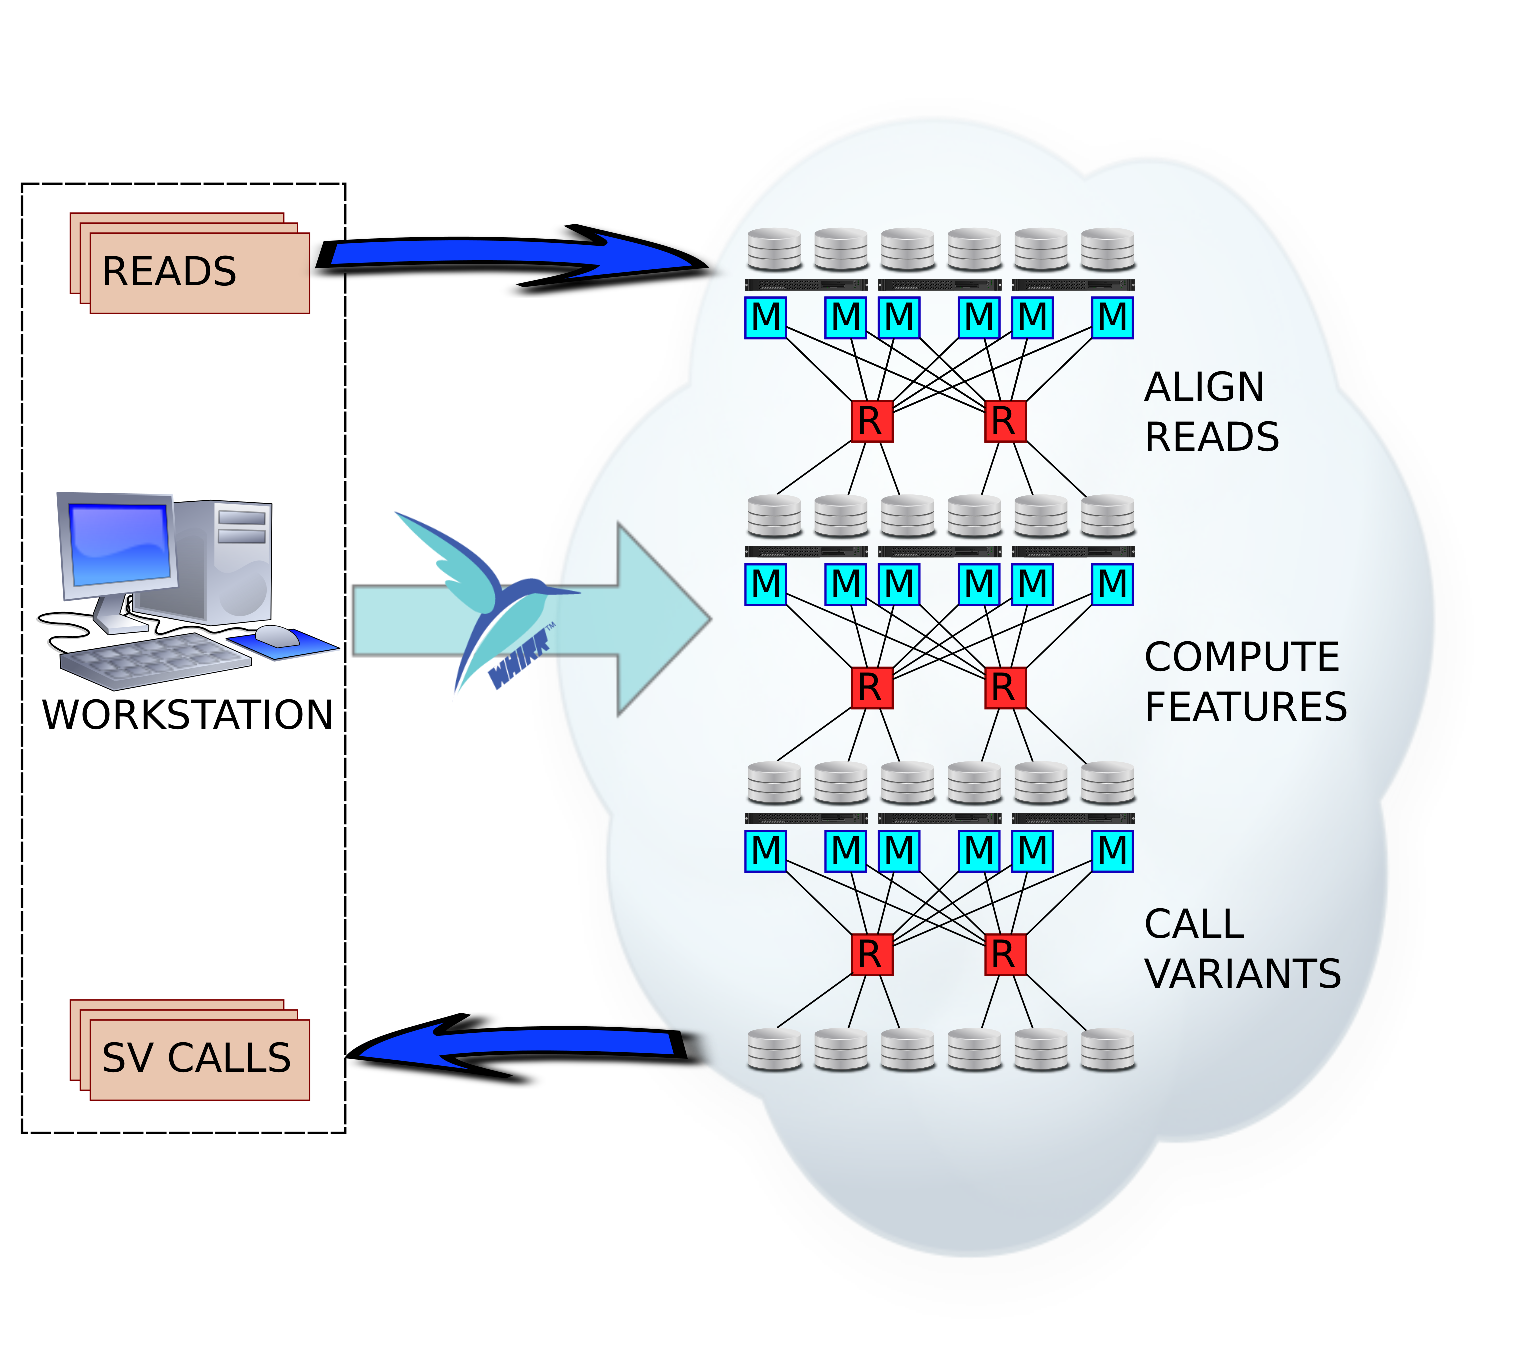
\includegraphics[width=.5\textwidth]{workflow_with_whirr.eps}
\caption{An overview of the Cloudbreak workflow. Reads are first uploaded to a Hadoop cluster from local storage. Cloudbreak then executes three MapReduce jobs to process the data: 1) Mapping with sensitive settings. 2) Computation of features across the genome. 3) Calling structural variations based on the features computed in the previous step. Finally, SV predictions can be downloaded from the Hadoop cluster and examined. Cloudbreak can also use the Apache Whirr library to automatically provision Hadoop clusters on and deploy data to cloud providers such as Amazon Elastic Compute Cloud.}
\label{cloudbreak_workflow}
\end{figure}

Our framework for SV detection in MapReduce divides processing into three distinct MapReduce jobs (Figure \ref{cloudbreak_workflow}): a job that can align reads to the reference using a variety of mapping algorithms; a job that computes a set of features along the genome; and a job which calls structural variations based on those features.

The \textsc{Align Reads} job uses existing alignment tools to discover mapping locations for each read pair. Aligners can be executed to report multiple possible mappings for each read, or only the best possible mapping. Given a set of read pairs, each of which consists of a read pair identifier $rpid$ and two sets of sequence and quality scores $<s,q>$, each mapper aligns each pair end set $<s,q>$ in either single- or paired end mode and emits possible mapping locations under the $rpid$ key. Reducers then collect the alignments for each paired end, making them available under one key for the next job. 

In the \textsc{Compute Features} job, we compute a set of features for each location in the genome. To begin, we tile the genome with small fixed-width, non-overlapping intervals. For the experiments reported below we use an interval size of 25bp (see Supplementary Materials for an exploration of the effects of different window sizes on accuracy and runtime). Let $L = \left\{l_1,l_2,\ldots,l_N\right\}$ be the set of intervals covering the entire genome. Let $R^1 = \left\{r^{1}_{1},r^{1}_{2},\ldots,r^{1}_{M}\right\}$ and $R^2 = \left\{r^{2}_{1},r^{2}_{2},\ldots,r^{2}_{M}\right\}$ be the input set of paired reads. Let $A^1 = \left\{a^{1}_{m,1},a^{1}_{m,2},\ldots,a^{1}_{m,K}\right\}$ and $A^2 = \left\{a^{2}_{m,1},a^{2}_{m,2},\ldots,a^{2}_{m,L}\right\}$ be the set of alignments for the left and right reads from read pair $m$. For any given pair of alignments of the two reads in a read pair, $a^{1}_{m,i}$ and $a^{2}_{m,j}$, let the $\textrm{ReadPairInfo } rpi_{m,i,j}$ be information about the pair relevant to detecting SVs, e.g. the fragment size implied by the alignments and the likelihood that the alignments are correct. We then leave two functions to be implemented depending on the application:
\begin{flalign*}
 \textsc{Loci } :& \langle a^{1}_{m,i},a^{2}_{m,j} \rangle \rightarrow L_m \subseteq L \\
 \Phi :& \left\{\textrm{ReadPairInfo }rpi_{m,i,j}\right\} \rightarrow \mathbb{R}^N 
\end{flalign*}

The first function, \textsc{Loci}, maps an alignment pair to a set of genomic locations to which it is relevant for SV detection; for example, the set of locations overlapped by the internal insert implied by the read alignments. We optimize this step by assuming that if there exist concordant mappings for a read pair, defined as those where the two alignments are in the proper orientation and with an insert size within three standard deviations of the expected library insert size, one of them is likely to be correct and therefore we do not consider any discordant alignments of the pair. The second function, $\Phi$, maps a set of ReadPairInfos relevant to a given location to a set of real-valued vectors of features useful for SV detection. 

Finally, the third MapReduce job, \textsc{Call Variants}, is responsible for making SV calls based on the features computed at each genomic location. It calls another application-specific function: 
 \[ \textsc{PostProcess} : \left\{\phi_1,\phi_2,\ldots,\phi_N\right\} \rightarrow \left\{\langle  \textrm{SVType } s, l_{start}, l_{end} \rangle\right\} \]

This function maps the sets of features for related loci into a set of SV calls characterized by their type $s$ (i.e Deletion, Insertion, etc.) and their breakpoint locations $l_{start}$ and $l_{end}$. We parallelize this job in MapReduce by making calls for each chromosome in parallel, which we achieve by associating a location and its set of features to its chromosome in the map phase, and then making SV calls for one chromosome in each reduce task.

\begin{algorithm}[t]
\algrenewcommand\algorithmicprocedure{\textbf{job}}
 \begin{algorithmic}[1]\raggedright
\footnotesize{
 \Procedure{Alignment}{}
 \Function{Map}{$\textrm{ReadPairId }rpid$, $\textrm{ReadId }r$, $\textrm{ReadSequence }s$, $\textrm{ReadQuality }q$}
 \ForAll{$ \textrm{Alignments }a \in \textsc{Align}(s,q)$}
 \State $\textsc{Emit}(\textrm{ReadPairId }rpid, \textrm{Alignment }a)$
 \EndFor
 \EndFunction
 \Function{Reduce}{$\textrm{ReadPairId }rpid, \textrm{Alignments }a_{1,2,\ldots}$}
 \State $\textrm{AlignmentPairList }ap \gets \textsc{ValidAlignmentPairs}(a_{1,2,\ldots})$
 \State $\textsc{Emit}(\textrm{ReadPairId }rp, \textrm{AlignmentPairList } ap)$
 \EndFunction
 \EndProcedure

 \Procedure{Compute SV Features}{}
 \Function{Map}{$\textrm{ReadPairId }rp, \textrm{AlignmentPairList }ap$}
 \ForAll{$ \textrm{AlignmentPairs }\langle a_1,a_2 \rangle \in ap$}
 \ForAll{$ \textrm{GenomicLoci }l \in \textsc{Loci }(a_1,a_2)$}
 \State $ \textrm{ReadPairInfo }rpi \gets \break\hspace*{2em} \langle\textrm{InsertSize}(a_1,a_2), \textrm{AlignScore}(a_1,a_2)\rangle$
 \State $\textsc{Emit}(\textrm{GenomicLocus }l, \textrm{ReadPairInfo }rpi)$
 \EndFor
 \EndFor
 \EndFunction
 \Function{Reduce}{$\textrm{GenomicLocus }l, \textrm{ReadPairInfos }rpi_{1,2,\ldots}$}
 \State $\textrm{SVFeatures } \phi_l \gets \Phi(\textrm{InsertSizes }i_{1,2,\ldots}, \textrm{AlignmentScores }q_{1,2,\ldots})$
 \State $\textsc{Emit}(\textrm{GenomicLocus }l, \textrm{SVFeatures } \phi_l)$
 \EndFunction
 \EndProcedure

 \Procedure{Call SVs}{}
 \Function{Map}{$\textrm{GenomicLocus }l, \textrm{SVFeatures } \phi_l$}
 \State $\textsc{Emit}(\textrm{Chromosome}(l), <l,\phi_l>)$
 \EndFunction
 \Function{Reduce}{$\textrm{Chromosome }c, \break \textrm{GenomicLocus } l_{1,2,\ldots}, \phi_{1,2,\ldots}$}
 \State $\textrm{StructuralVariationCalls } svs_c \gets \textsc{PostProcess }(\phi_{1,2,\ldots})$
 \EndFunction
 \EndProcedure
}
 \end{algorithmic}
\caption{A framework for SV calling in MapReduce.}
\label{cb_algo}
\end{algorithm}

\subsection{Cloudbreak: Detecting Deletions and Insertions}

We have implemented an RP-based SV detection package, Cloudbreak, in the framework described above. Cloudbreak detects deletions of size 40bp to 25kb, and small insertions. We accomplish this by providing the following implementations of the user-defined functions described above:

\textbf{\sc{Loci}}: Because we are detecting deletions and short insertions, we map ReadPairInfos from each possible alignment to the genomic locations overlapped by the implied internal insert between the reads. For efficiency, we define a maximum detectable deletion size of 25,000bp, and therefore alignment pairs in which the ends are more than 25kb apart, or in the incorrect orientation, map to no genomic locations.

\textbf{$\Phi$}: To compute features for each genomic location, we follow \cite{Lee:2009da}, who observed that if all mappings are correct, the insert sizes implied by mappings which span a given genomic location should follow a Gaussian mixture model (GMM) whose parameters depend on whether a deletion or insertion is present at that locus (Supplementary Figure 1\todo{\ref{Sinsert_size_mixes}}). Briefly: if there is no indel, the insert sizes implied by spanning alignment pairs should follow the distribution of actual fragment sizes in the sample, which is typically modeled as normally distributed with mean $\mu$ and standard deviation $\sigma$. If there is a homozygous deletion or insertion of length $l$ at the location, $\mu$ should be shifted to $\mu + l$, while $\sigma$ will remain constant. Finally, in the case of a heterozygous event, the distribution of insert sizes will follow a mixture of two normal distributions, one with mean $\mu$, and the other with mean $\mu + l$, both with an unchanged standard deviation of $\sigma$, and mixing parameter $\alpha$ that describes the relative weights of the two components. Because the mean and standard deviation of the fragment sizes are selected by the experimenter and therefore known \emph{a priori} (or at least easily estimated based on a sample of alignments), we only need to estimate the mean of the second component at each locus, and the mixing parameter $\alpha$. We fit these parameters using an Expectation-Maximization algorithm (see Supplementary Material). To remove incorrect mappings, we use an adaptive quality cutoff for each genomic location and then perform an outlier-detection based noise reduction technique; these procedures also allow us to process multiple mappings for each read if they are reported by the aligner (see Supplementary Material). The features generated for each location $l$ include the log-likelihood ratio of the filtered observed data points under the fit GMM to their likelihood under the distribution $N(\mu,\sigma)$, the final value of the mixing parameter $\alpha$, and $\mu'$, the estimated mean of the second GMM component.

\textbf{\sc{PostProcess}}: We convert our features along each chromosome to insertion and deletion calls by first extracting contiguous genomic loci where the log-likelihood ratio of the two models is greater than a given threshold. To eliminate noise we apply a median filter. We end regions when $\mu'$ changes by more than $2\sigma$, and discard regions where the average value of $\mu'$ is less than $\mu$ or where the length of the region differs from $\mu'$ by more than $\mu$.

An illustration of the Cloudbreak algorithm working on a simple example is shown in Supplementary Figure 2\todo{\ref{Salgorithm_example}}.

\subsection{Implementation Details}

Cloudbreak is a native Java Hadoop application. We deployed Cloudbreak on a 56-node cluster running the Cloudera CDH3 Hadoop distribution, version 0.20.2-cdh3u4. We use snappy compression for MapReduce data. Hadoop's distributed cache mechanism shares the executable files and indices needed for mapping tasks to the nodes in the cluster. 

Cloudbreak's alignment job can run a variety of alignment tools that report reads in SAM format (Supplementary Materials). In the map phase, mappers align reads in either single-end or paired-end mode to the reference genome in parallel, outputting mapping locations as values under a key identifying the read pair. In the reduce phase, the framework combines the reported mapping locations for the two ends of each read pair. This job can also be skipped in favor of importing a pre-existing set of mappings directly into the Hadoop cluster.

\subsection{Cloudbreak Genotyping}
We used the parameters of the fit GMM to infer the genotype of each predicted variant. Assuming that our pipeline is capturing all relevant read mappings near the locus of the variant, the genotype should be indicated by the estimated parameter $\alpha$, the mixing parameter that controls the weight of the two components in the GMM. By tuning on the simulated data, we determined that by setting a simple cutoff of .35 on the average value of $\alpha$ for each prediction, we were able to accurately (see Section~\ref{section_results_genotyping}) call the predicted variant homozygous or heterozygous. We used the same cutoff for deletion and insertion predictions.

\subsection{Running Locally or in the Cloud}

Cloudbreak can be executed on any Hadoop cluster; Hadoop abstracts away the details of cluster configuration, making distributed applications portable. In addition, our Cloudbreak implementation can leverage the Apache Whirr library to automatically create clusters with cloud service providers such as the Amazon Elastic Compute Cloud (EC2). This enables on demand provisioning of Hadoop clusters which can then be terminated when processing is complete, eliminating the need to invest in a standing cluster and allowing a model in which users can scale their computational infrastructure as their need for it varies over time. In addition, Whirr supports multiple cloud service providers, making it possible to leverage many public or private clouds and avoid vendor lock-in. Instructions and examples describing how to leverage cloud computing with Cloudbreak are available in the user manual and Supplementary Materials.

% \begin{table}[!t]
% \processtable{This is table caption\label{Tab:01}}
% {\begin{tabular}{llll}\toprule
% head1 & head2 & head3 & head4\\\midrule
% row1 & row1 & row1 & row1\\
% row2 & row2 & row2 & row2\\
% row3 & row3 & row3 & row3\\
% row4 & row4 & row4 & row4\\\botrule
% \end{tabular}}{This is a footnote}
% \end{table}

\end{methods}

% \begin{figure}[!tpb]%figure1
% %\centerline{\includegraphics{fig01.eps}}
% \caption{Caption, caption.}\label{fig:01}
% \end{figure}

% \begin{figure}[!tpb]%figure2
% %\centerline{\includegraphics{fig02.eps}}
% \caption{Caption, caption.}\label{fig:02}
% \end{figure}

\section{Results}

\subsection{Tests with Simulated Data}

We compared the performance of Cloudbreak for detecting deletions and insertions to a selection of popular tools: the RP method BreakDancer~\citep{Chen:2009p3}, GASVPro, an RP method that integrates RD signals and ambiguous mappings~\citep{Sindi:2012kk}, the SR method Pindel~\citep{Ye:2009p2}, and the hybrid RP-SR method DELLY~\citep{Rausch:2012he}. DELLY produces two sets of calls, one based solely on RP signals, and the other based on RP calls that could be supported by SR evidence; we refer to these sets of calls as DELLY-RP and DELLY-SR. We also attempted to evaluate MoDIL on the same data. All of these methods detect deletions. Insertions can be detected by BreakDancer, Pindel, and MoDIL. See Supplementary Materials for details on how reads were aligned and each program was invoked. For all alignments we used BWA~\citep{Li:2009p836}, although in testing Cloudbreak we have found that the choice of aligner, number of possible mapping locations reported, and whether the reads were aligned in paired-end or single-ended mode can have a variety of effects on the output of the algorithm (Supplementary Fig. 3\todo{\ref{Salignment_comparison}}).

There is no available test set of real Illumina sequencing data from a sample that has a complete annotation of SVs. Therefore, testing with simulated data is important to fully characterize an algorithm's performance characteristics. On the other hand, any simulated data should contain realistic SVs that follow patterns observed in real data. We took one of the most complete lists of SVs from an individual, the list of homozygous insertions and deletions from the genome of J. Craig Venter~\citep{Levy:2007fb}, and used it to simulate a 30X read coverage data set for a diploid human Chromosome 2 with a mix of homozygous and heterozygous variants, with 100bp reads and a mean fragment size of 300bp (See Supplementary Material).

\begin{figure*}[!tpb]
\centering
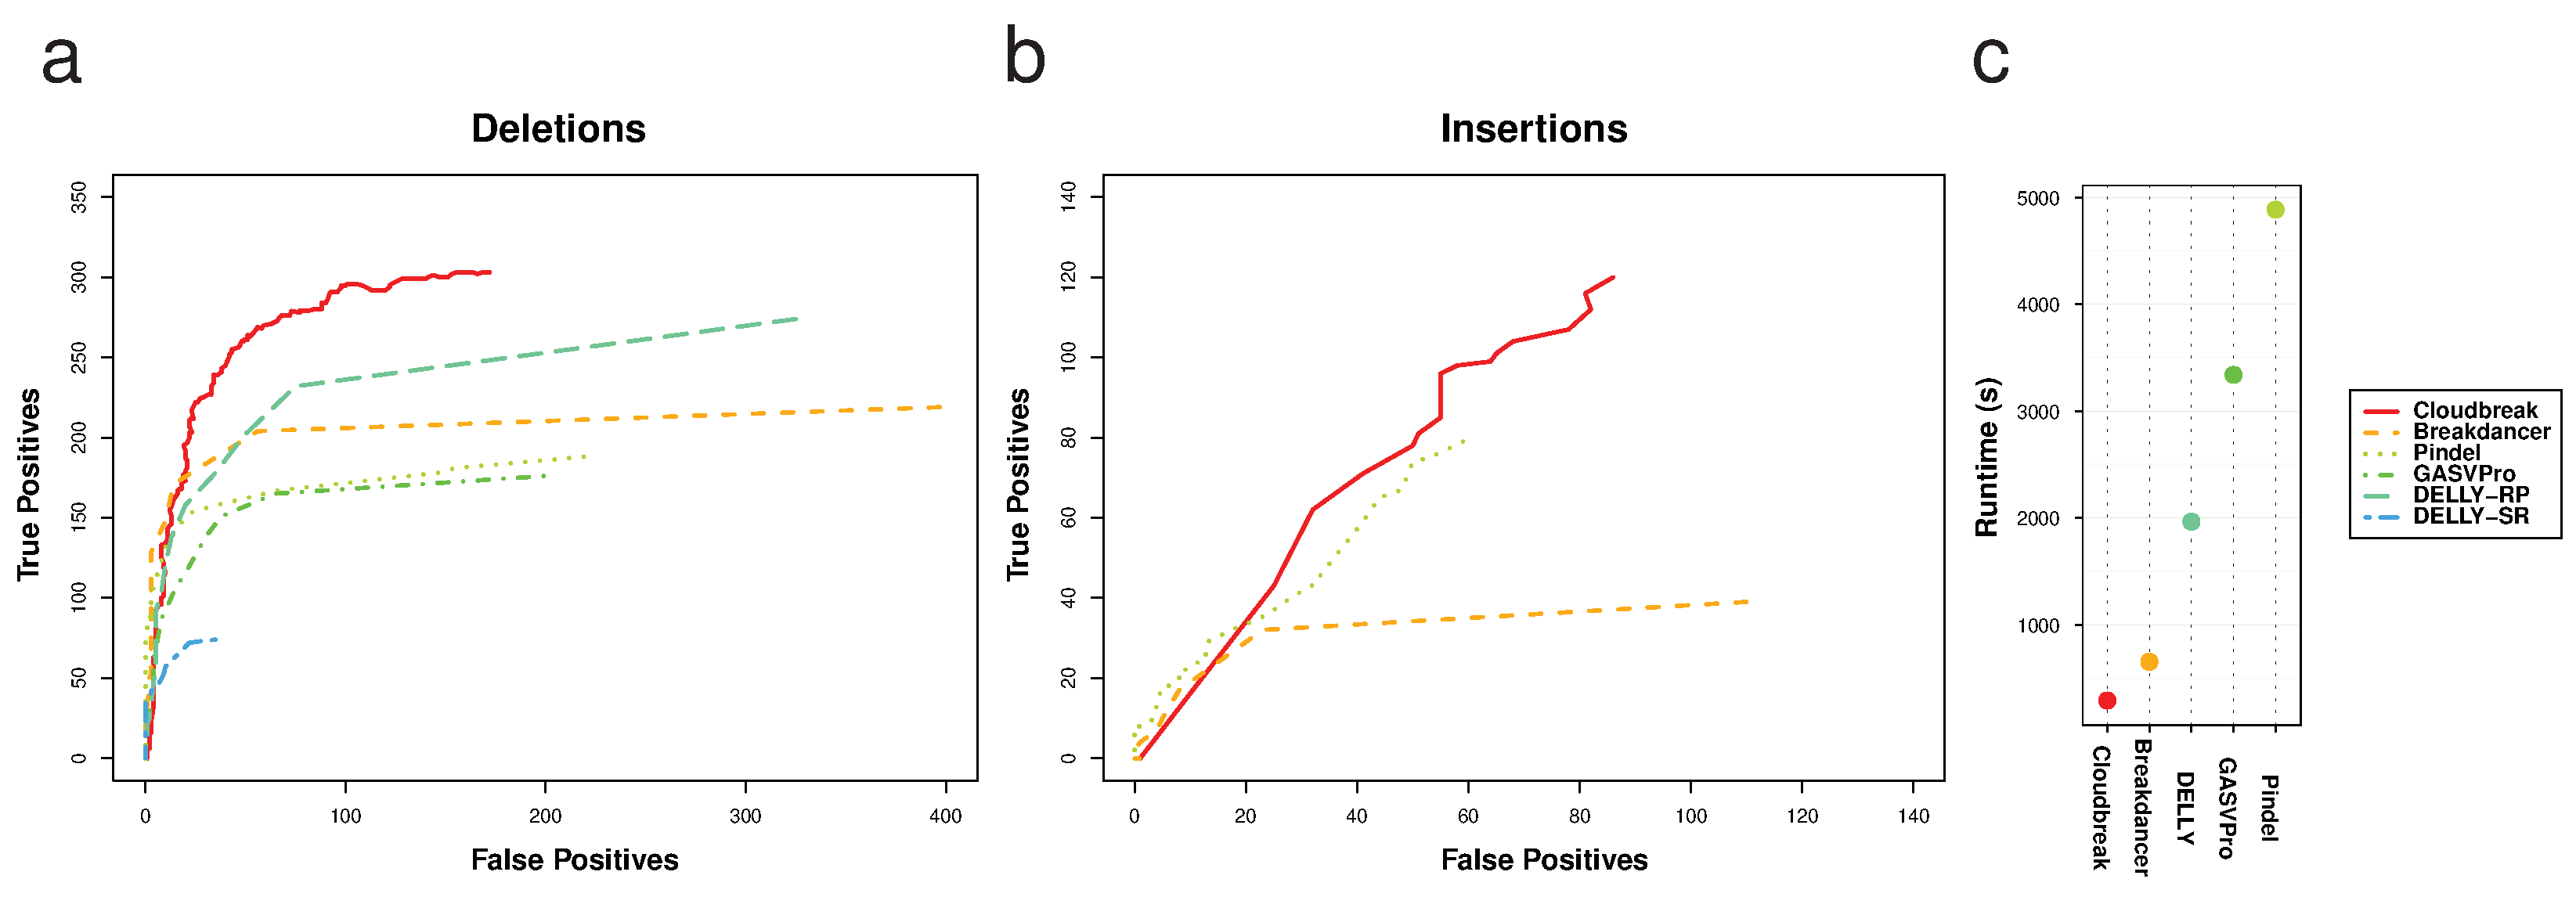
\includegraphics[width=1\textwidth]{chr2_rocs_runtimes_journal.eps}
\caption{Accuracy and runtime performance on a simulated data set. (a) Receiver Operating Characteristic (ROC) curves showing the specificity and sensitivity of each tool to deletions larger than 40bp on a simulated set of reads giving diploid coverage of 30X on human chromosome 2. Deletions from the Venter genome were randomly added to one or both haplotypes. Each point on a curve represents a different threshold on the confidence of predictions made by that tool. Thresholds vary by: Cloudbreak - likelihood ratio; BreakDancer, DELLY, GASVPro - number of supporting read pairs; Pindel - simple score. (b) ROC curves for insertion predictions. (c) Runtimes for each tool, not including alignment time, parallelized when possible (see Supplementary Material).}
\label{chr2CombinedRoc}
\end{figure*}

Figure \ref{chr2CombinedRoc} shows Receiver Operating Characteristic (ROC) curves of the performance of each algorithm at identifying variants larger than 40bp on the simulated data set, as well as the runtimes of the approaches tested, excluding alignment. See Supplementary Material for a description of how we identified correct predictions. All approaches show high specificity to deletions at stringent thresholds in this simulation. If specificity is relaxed slightly, Cloudbreak provides the highest levels of sensitivity, followed by DELLY. For insertions, Cloudbreak's performance is similar to Pindel, although Cloudbreak can achieve greater sensitivity at the same false positive rate by decreasing its threshold. Cloudbreak's runtime is half that of BreakDancer, the next fastest tool, processing the simulated data in under six minutes. (Of course, Cloudbreak uses many more CPUs as distributed algorithm. See Supplementary Material and Supplementary Table 1 for a discussion of runtimes and parallelization.) The output which we obtained from MoDIL did not have a threshold that could be varied to correlate with the trade-off between precision and recall and therefore it is not included in ROC curves; in addition, MoDIL ran for 52,547 seconds using 250 CPUs. Apart from the alignment phase, which is embarrassingly parallel, the feature generation job is the most computationally intensive part of the Cloudbreak workflow. To test its scalability we measured its runtime on Hadoop clusters made up of varying numbers of nodes and observed that linear speedups can be achieved in this portion of the algorithm by adding additional nodes until a point of diminishing returns is reached (Supplementary Fig. 4\todo{\ref{Sscalability}}).

Choosing the correct threshold to set on the output of an SV calling algorithm can be difficult. The use of simulated data and ROC curves allows for some investigation of the performance characteristics of algorithms at varying thresholds. First, we characterized the predictions made by each algorithm at the threshold that gives them maximum sensitivity. The results are summarized in Table \ref{chr2DeletionAndInsertionPredsMaxSensitivity}. MoDIL and Cloudbreak exhibited the greatest recall for deletions. Cloudbreak also has high precision at this threshold, and discovers many small variants. For insertions, Cloudbreak has the highest recall, although recall is low for all four approaches. Cloudbreak again identifies many small variants. Pindel is the only tool which can consistently identify large insertions, as insertions larger than the library insert size do not produce mapping signatures detectable by RP mapping. We also used the ROC curves to characterize algorithm performance when a low false discovery rate is required. Supplementary Table 2\todo{\ref{Schr2DeletionPredsFDR10}} shows the total number of deletions found when choosing a threshold that gives an FDR closest to 10\% based on the ROC curve. At this more stringent cutoff, Cloudbreak identifies more deletions in every size category than any other tool. Insertion performance never reached an FDR of 10\% for any threshold, so insertion predictions are not included in this table.

We designed Cloudbreak to optimize for sensitivity and specificity for SV events, as demonstrated in the ROC curves, as opposed to attempting to achieve high levels of breakpoint resolution. Supplementary Fig. 5\todo{\ref{Sbreakpoint_resolution}} displays the breakpoint resolution of each of the methods tested on the simulated data set. Cloudbreak's resolution is lower than other methods because the independent calculation of features at each window does not allow the algorithm to keep track of the actual coordinates of the mapped reads from each pair, which other tools use to set bounds on the true breakpoint locations. In practice, RP-based predictions are typically validated using techniques such as targeted split read search, local assembly, or wet-lab methods, processes which refine their breakpoint predictions. Therefore, Cloudbreak attempts to maximize the accurate detection of the presence of SV events.

\begin{table*}[b]
\begin{center}
%\resizebox{\textwidth}{!}{
\footnotesize
\begin{tabular}{r|rrrr|rrrrr}
  \cline{2-10}
   &                     & Prec. & Recall & F1 & 40-100bp  & 101-250bp  & 251-500bp & 501-1000bp & $>$ 1000bp \\ 
\hline
\multirow{7}{*}{\begin{sideways}Deletions\end{sideways}} & Total Number &          &           &  &  224 &  84 & 82 &  31 & 26\\ 
  \hline
\cline{2-10}
&  Cloudbreak    &  0.638 & \textbf{0.678} & \textbf{0.657} & \textbf{153} (9)  & 61 (0) &  62 (0) & 12 (0) & 15 (0) \\ 
&  BreakDancer   &  0.356 & 0.49 & 0.412 & 89 (0)  & 54 (0) &  53 (0) & 8 (0) & 15 (0) \\ 
&  GASVPro        & 0.146 & 0.432 & 0.218 & 83 (2)  & 32 (0) &  55 (0) & 8 (0) & 15 (0) \\ 
&  DELLY-RP           & 0.457 & 0.613 & 0.613 & 114 (3)  & \textbf{68} (0) &  \textbf{66} (0) & 9 (1) & 17 (0) \\ 
&  DELLY-SR           & \textbf{0.679} & 0.166 &  0.266 & 0 (0)  & 3 (0) &  49 (0) & 6 (0) & 16 (0) \\ 
&  Pindel           & 0.462 & 0.421 &  0.44 & 96 (\textbf{11})  & 24 (0) &  48 (0) & 5 (0) & 15 (0)\\ 
&  MoDIL           & 0.132  & 0.66 & 0.22 & 123 (6)  & 66 (\textbf{3}) &  \textbf{66} (\textbf{11}) & \textbf{17} (\textbf{7}) & \textbf{23} (\textbf{8})\\ 
   \hline
\multirow{5}{*}{\begin{sideways}Insertions\end{sideways}} & Total Number &          &           & & 199 &  83 & 79 &  21 & 21\\ 
\cline{2-10}
&  Cloudbreak   &0.451 & \textbf{0.305}  & \textbf{0.364}  & \textbf{79} (\textbf{32})  & \textbf{32} (\textbf{18}) &  \textbf{11} (8) & 1 (0) & 0 (0) \\ 
&  BreakDancer & 0.262 & 0.0968  & 0.141  & 23 (5)  & 14 (5) &  2 (1) & 0 (0) & 0 (0) \\ 
&  Pindel          & \textbf{0.572} & 0.196 &  0.292 & 52 (25)  & 5 (1) &  10 (\textbf{9}) & \textbf{3} (\textbf{2}) & \textbf{9} (\textbf{9})\\ 
&  MoDIL          & 0.186 & 0.0521 &  0.0814 & 14 (1)  & 4 (0) &  1 (0) & 2 (\textbf{2}) & 0 (0)\\ 
\hline
\end{tabular}
%}
\end{center}
\caption{The number of simulated deletions and insertions in the 30X diploid chromosome 2 with Venter indels found by each tool at maximum sensitivity, as well as the number of those variants that were discovered exclusively by each tool (in parentheses). The total number of variants in each size class in the true set of deletions and insertions is shown in the first row of each section.}
\label{chr2DeletionAndInsertionPredsMaxSensitivity}
\end{table*}

\subsection{Tests with Biological Data}

We downloaded a set of reads from Yoruban individual NA18507, experiment ERX009609, from the Sequence Read Archive. This sample was sequenced by Illumina Inc. on the Genome Analyzer II platform with 100bp paired end reads and a mean fragment size (minus adapters) of 300bp, with a standard deviation of 15bp, to a depth of approximately 37X coverage. To create a gold standard set of insertions and deletions to test against, we pooled annotated variants discovered by three previous studies on the same individual. These included data from the Human Genome Structural Variation Project reported by~\cite{Kidd:2008p926}, a survey of small indels conducted by~\cite{Mills:2011fi}, and insertions and deletions from the merged call set of the phase 1 release of the 1000 Genomes Project~\citep{GenomesProjectConsortium:2012co} which were genotyped as present in NA18507. We merged any overlapping calls of the same type into the region spanned by their unions. We were unable to run MoDIL on the whole-genome data set due to the estimated runtime and storage requirements.

\begin{figure*}
\centering
\includegraphics[width=1\textwidth]{NA18507_rocs_runtimes_journal.eps}
\caption{Accuracy and performance on the 37X NA18507 sample. (a) ROC curve for deletion prediction performance, tested against the combined gold standard sets of deletions taken from~\cite{Kidd:2008p926},~\cite{Mills:2011fi}, and~\cite{GenomesProjectConsortium:2012co}. (b) ROC curve for insertion prediction performance. (c) Runtimes for each tool, not including alignment time, parallelized when possible (see Supplementary Material). }
\label{NA18507CombinedRoc}
\end{figure*}

Figure \ref{NA18507CombinedRoc} shows the performance of each algorithm on the NA18507 data set. All algorithms show far less specificity for the gold standard set than they did in the single chromosome simulation, although it is difficult to tell how much of the difference is due to the added complexity of real data and a whole genome, and how much is due to missing variants in the gold standard set that are actually present in the sample. For deletions, Cloudbreak is the best performer at the most stringent thresholds, and has the highest or second highest precision at higher sensitivity levels. Cloudbreak has comparable accuracy for insertions to other tools, and can identify the most variants at higher levels of sensitivity. Cloudbreak processes the sample in under 15 minutes on our cluster, more than six times as fast as the next fastest program, BreakDancer, even when BreakDancer is run in parallel for each chromosome on different nodes in the cluster.

Given the high number of novel predictions made by all tools at maximum sensitivity, we decided to characterize performance at more stringent thresholds. We examined the deletion predictions made by each algorithm using the same cutoffs that yielded a 10\% FDR on the simulated chromosome 2 data set, adjusted proportionally for the difference in coverage from 30X to 37X. For insertions, we used the maximum sensitivity thresholds for each tool due to the high observed FDRs in the simulated data. Precision and recall at these thresholds, as well as the performance of each algorithm at predicting variants of each size class, is shown in Table \ref{NA18507DeletionAndInsertionPreds}. For deletions, Cloudbreak has the greatest sensitivity of any tool, identifying the most variants in each size class. Pindel exhibits the highest precision with respect to the gold standard set. For insertions, Pindel again has the highest precision at maximum sensitivity, while Cloudbreak has by far the highest recall.

\begin{table*}
\begin{center}
%\resizebox{\textwidth}{!}{
\footnotesize
\begin{tabular}{r|rrrr|rrrrr}
  \cline{2-10}
&  & Prec. & Recall & F1 & 40-100bp & 101-250bp & 251-500bp & 501-1000bp & $>$ 1000bp \\ 
\hline
\multirow{6}{*}{\begin{sideways}Deletions\end{sideways}} & Total Number & & & & 7,462 & 240 & 232 & 147 & 540 \\
  \hline
\cline{2-10}
& Cloudbreak & 0.0943 & \textbf{0.17} & 0.121 & \textbf{573} (\textbf{277})  & \textbf{176} (\textbf{30}) &  \textbf{197} (\textbf{18}) & \textbf{121} (\textbf{6}) & \textbf{399} (\textbf{24}) \\ 
& BreakDancer & 0.137 & 0.123 &  \textbf{0.13} & 261 (29)  & 136 (3) &  178 (0) & 114 (0) & 371 (0) \\  
&  GASVPro & 0.147 & 0.0474 &  0.0717 & 120 (21)  & 40 (2) &  85 (0) & 36 (0) & 128 (0) \\ 
&  DELLY-RP & 0.0931 & 0.1 &  0.0965 & 143 (6)  & 128 (3) &  167 (1) & 103 (0) & 323 (1) \\ 
&  DELLY-SR & 0.153 & 0.0485 &  0.0736 & 0 (0)  & 26 (0) &  123 (0) & 66 (0) & 203 (0) \\ 
&  Pindel & \textbf{0.179} & 0.0748 &  0.106 & 149 (8)  & 61 (0) &  149 (0) & 69 (1) & 217 (0) \\ 
\hline
\multirow{4}{*}{\begin{sideways}Insertions\end{sideways}} & Total Number & & & & 536 & 114 & 45 & 1 & 0 \\
\cline{2-10}
& Cloudbreak & 0.0323 & \textbf{0.455} &  0.0604 & \textbf{265} (\textbf{104})  & \textbf{49} (\textbf{24}) &  3 (1) & 0 (0)  & 0 (0)  \\ 
& BreakDancer & 0.0281 & 0.181 &  0.0487 & 97 (10)  & 27 (5) &  2 (1) & 0 (0) & 0 (0) \\  
&  Pindel & \textbf{0.0387} & 0.239 &  \textbf{0.0666} & 144 (45)  & 14 (7) &  \textbf{7} (\textbf{6}) & \textbf{1} (\textbf{1}) &  0 (0) \\ 
\hline
\end{tabular}
%}
\end{center}
\caption{The precision and recall with respect to the gold standard set of deletions and insertions for each tool on the NA18507 data, as well as the number of variants found in each size class found. Exclusive predictions are in parentheses. For deletions, the same cutoffs were used as for the simulated data as in Supplementary Table 2\todo{\ref{Schr2DeletionPredsFDR10}}, adjusted for the difference in coverage from 30X to 37X. For insertions, the maximum sensitivity cutoff was used.}
\label{NA18507DeletionAndInsertionPreds}
\end{table*}

\subsection{Performance on a Low-Coverage Cancer Data Set}

We also tested Cloudbreak on a data set obtained from a patient with acute myeloid leukemia (AML). This data consisted of 76bp paired end reads with a mean insert size of 285bp and standard deviation of 50bp, yielding sequence coverage of 5X and physical coverage of 8X. Using a pipeline consisting of Novoalign, BreakDancer, and a set of custom scripts for filtering and annotating candidate SVs, we had previously identified a set of variants present in this sample and validated several using PCR, including 8 deletions. Cloudbreak was able to identify all of the validated deletions, showing that it is still sensitive even when using lower coverage data with a greater variance of insert sizes. The variants identified include deletions in the gene \emph{CTDSPL}/\emph{RBPS3}, an AML tumor suppressor~\citep{Zheng:2012kk}, and NBEAL1, a gene up-regulated in some cancers~\citep{Chen:2004jo}. We are currently investigating these SVs to determine their functional impact on this patient. 

\subsection{Genotyping Deletions}\label{section_results_genotyping}

Because Cloudbreak explicitly models zygosity in its feature generation algorithm, it can predict the genotypes of identified variants. We tested this on both the simulated and NA18507 data sets. For the NA18507 data set, we considered the deletions from the 1000 Genomes Project, which had been genotyped using the population-scale SV detection algorithm Genome STRiP~\citep{Handsaker:2011ki}. Cloudbreak was able to achieve 92.7\% and 95.9\% accuracy in predicting the genotype of the deletions it detected at our 10\% FDR threshold in the simulated and real data sets, respectively. Supplementary Table 3\todo{\ref{SdeletionGenotypeaccuracy}} shows confusion matrices for the two samples using this classifier. \todo{None of the three input sets that made up the gold standard for NA18507 contained a sufficient number of insertions that met our size threshold and also had genotyping information. Of the 123 insertions detected by Cloudbreak on the simulated data set, 43 were heterozygous. Cloudbreak correctly classified 78 of the 80 homozygous insertions and 31 of the 43 heterozygous insertions, for an overall accuracy of 88.6\%.}

\section{Discussion}

Over the next few years, due to advances in sequencing technology, genomics data are expected to increase in volume by several orders of magnitude, expanding into the realm referred to as ``big data''. In addition, the usage of existing information will increase drastically as research in genomics grows and translational applications are developed, and data is reprocessed and integrated into new pipelines. In order to capitalize on this emerging wealth of genome data, novel computational solutions that are capable of scaling with the increasing number and size of these data sets will have to be developed. 

Among big data infrastructures, MapReduce is emerging as a standard framework for distributing computation across compute clusters. In this paper, we introduced a novel conceptual framework for SV detection algorithms in MapReduce, based on computing local genomic features. This framework provides a scalable basis for developing SV detection algorithms, as demonstrated by our development of an algorithm for detecting insertions and deletions based on fitting a GMM to the distribution of mapped insert sizes spanning each genomic location.

On simulated and real data sets, our approach exhibits high accuracy when compared to popular SV detection algorithms that run on traditional clusters and servers. Detection of insertions and deletions is an important area of research; \cite{Mills:2011fi} recently identified over 220 coding deletions in a survey of a large number of individuals, and they note that such variants are likely to cause phenotypic variation in humans. 

In addition to delivering high accuracy and fast runtimes for a RP-based SV detection tool, our approach offers a basis for developing a variety of SV algorithms can run in MapReduce pipelines with the power to process vast amounts of data in a cloud or commodity server setting. With the advent of cloud service providers such as Amazon EC2, it is becoming easy to instantiate on-demand Hadoop compute clusters. Having computational approaches that can harness this capability will become increasingly important for researchers or clinicians who need to analyze increasing amounts of sequencing data.

% Text Text Text Text Text Text  Text Text Text Text Text Text Text Text Text  Text Text Text Text Text Text. Figure \ref{fig:02} shows that the above method  Text Text Text Text  Text Text Text Text Text Text  Text Text.  \citepalp{Boffelli03} might want to know about  text text text text
% Text Text Text Text Text Text  Text Text Text Text Text Text Text Text Text  Text Text Text Text Text Text. Figure \ref{fig:02} shows that the above method  Text Text Text Text  Text Text Text Text Text Text  Text Text.  \citepalp{Boffelli03} might want to know about  text text text text
% Text Text Text Text Text Text  Text Text Text Text.




% Table~\ref{Tab:01} shows that Text Text Text Text Text  Text Text Text Text Text Text. Figure \ref{fig:02} shows that
% the above method Text Text. Text Text Text  Text Text Text Text Text Text. Figure \ref{fig:02} shows that
% the above method Text Text. Text Text Text  Text Text Text Text Text Text. Figure \ref{fig:02} shows that
% the above method Text Text.









%%%%%%%%%%%%%%%%%%%%%%%%%%%%%%%%%%%%%%%%%%%%%%%%%%%%%%%%%%%%%%%%%%%%%%%%%%%%%%%%%%%%%
%
%     please remove the " % " symbol from \centerline{\includegraphics{fig01.eps}}
%     as it may ignore the figures.
%
%%%%%%%%%%%%%%%%%%%%%%%%%%%%%%%%%%%%%%%%%%%%%%%%%%%%%%%%%%%%%%%%%%%%%%%%%%%%%%%%%%%%%%






\section{Conclusion}

% (Table~\ref{Tab:01}) Text Text Text Text Text Text  Text Text Text Text Text Text Text Text Text  Text Text Text Text Text Text. Figure \ref{fig:02} shows that the above method  Text Text Text Text  Text Text Text Text Text Text  Text Text.  \citepalp{Boffelli03} might want to know about  text text text text
% Text Text Text Text Text Text  Text Text Text Text Text Text Text Text Text  Text Text Text Text Text Text. Figure \ref{fig:02} shows that the above method  Text Text Text Text  Text Text Text Text Text Text  Text Text.  \citepalp{Boffelli03} might want to know about  text text text text
% Text Text Text Text Text Text  Text Text Text Text Text Text Text Text Text  Text Text Text Text Text Text. Figure \ref{fig:02} shows that the above method  Text Text Text Text  Text Text Text Text Text Text  Text Text.



% Text Text Text Text Text Text  Text Text Text Text Text Text Text Text Text  Text Text Text Text Text Text. Figure \ref{fig:02} shows that the above method  Text Text Text Text  Text Text Text Text Text Text  Text Text.  \citepalp{Boffelli03} might want to know about  text text text text





% \begin{enumerate}
% \item this is item, use enumerate
% \item this is item, use enumerate
% \item this is item, use enumerate
% \end{enumerate}

% Text Text Text Text Text Text  Text Text Text Text Text Text Text Text Text  Text Text Text Text Text Text. Figure \ref{fig:02} shows that the above method  Text Text Text Text  Text Text Text Text Text Text  Text Text.  \citepalp{Boffelli03} might want to know about  text text text text
% Text Text Text Text Text Text  Text Text Text Text Text Text Text Text Text  Text Text Text Text Text Text. Figure \ref{fig:02} shows that the above method  Text Text Text Text  Text Text Text Text Text Text  Text Text.  \citepalp{Boffelli03} might want to know about  text text text text
% Text Text Text Text Text Text  Text Text Text Text Text Text Text Text Text  Text Text Text Text Text Text.






% Text Text Text Text Text Text  Text Text Text Text Text Text Text Text Text  Text Text Text Text Text Text. Figure \ref{fig:02} shows that the above method  Text Text Text Text


\section*{Acknowledgement}
We thank Izhak Shafran at the Center for Spoken Language Understanding for advice, support, and shared computational resources, and Bob Handsaker for helpful conversations.

\paragraph{Funding\textcolon} C.T.S. and A.L.A. are supported by the Italian Association for Cancer Research (AIRC). Sequencing of the AML sample was supported by the Oregon Medical Research Foundation. 

\bibliographystyle{natbib}
%\bibliographystyle{achemnat}
%\bibliographystyle{plainnat}
%\bibliographystyle{abbrv}
%\bibliographystyle{bioinformatics}
%
%\bibliographystyle{plain}
%
\bibliography{Document}


% \begin{thebibliography}{}
% \bibitem[Bofelli {\it et~al}., 2000]{Boffelli03} Bofelli,F., Name2, Name3 (2003) Article title, {\it Journal Name}, {\bf 199}, 133-154.

% \bibitem[Bag {\it et~al}., 2001]{Bag01} Bag,M., Name2, Name3 (2001) Article title, {\it Journal Name}, {\bf 99}, 33-54.

% \bibitem[Yoo \textit{et~al}., 2003]{Yoo03}
% Yoo,M.S. \textit{et~al}. (2003) Oxidative stress regulated genes
% in nigral dopaminergic neurnol cell: correlation with the known
% pathology in Parkinson's disease. \textit{Brain Res. Mol. Brain
% Res.}, \textbf{110}(Suppl. 1), 76--84.

% \bibitem[Lehmann, 1986]{Leh86}
% Lehmann,E.L. (1986) Chapter title. \textit{Book Title}. Vol.~1, 2nd edn. Springer-Verlag, New York.

% \bibitem[Crenshaw and Jones, 2003]{Cre03}
% Crenshaw, B.,III, and Jones, W.B.,Jr (2003) The future of clinical
% cancer management: one tumor, one chip. \textit{Bioinformatics},
% doi:10.1093/bioinformatics/btn000.

% \bibitem[Auhtor \textit{et~al}. (2000)]{Aut00}
% Auhtor,A.B. \textit{et~al}. (2000) Chapter title. In Smith, A.C.
% (ed.), \textit{Book Title}, 2nd edn. Publisher, Location, Vol. 1, pp.
% ???--???.

% \bibitem[Bardet, 1920]{Bar20}
% Bardet, G. (1920) Sur un syndrome d'obesite infantile avec
% polydactylie et retinite pigmentaire (contribution a l'etude des
% formes cliniques 
% @article{Dean:2008p277,
% author = {Dean, J and Ghemawat, S},
% title = {{MapReduce: Simplified data processing on large clusters}},
% journal = {Commun. ACM},
% year = {2008},
% volume = {51},
% number = {1},
% pages = {107--113}
% }
% de l'obesite hypophysaire). PhD Thesis, name of
% institution, Paris, France.

% \end{thebibliography}
\end{document}
